\chapter{Inflationary Fluctuations And The Origin Of Structure}

This lecture opens with what looks at first like a detour. Before Leonard Susskind turns to inflation, he spends a long time separating universal constants from the many contingent parameters of low-energy physics, and he uses that separation to build the Planck units. That prelude is not ornamental. It sets the hierarchy of scales for everything that follows. Only then do we come to the cosmological puzzle itself: the universe is extraordinarily smooth, but not perfectly smooth, and those tiny departures from homogeneity are the seeds of the structure we see today. These notes follow the lecture closely, using selected blackboard evidence preserved through LazyingArt LLC and Video2Book whenever the board itself carries part of the reasoning.

\section{Universal Constants And Planck Units}

The lecture begins with a contrast. The standard model is a highly accurate description of elementary particles, but it contains many parameters: masses, couplings, charges, mixing angles, and the very list of particles. Those numbers are real, but they do not look universal. By comparison, three constants stand out as applying to everything: the speed of light \(c\), Planck's constant \(\hbar\), and Newton's constant \(G\). Susskind's criterion is simple: whenever a law says \emph{all} objects, \emph{all} matter, or \emph{all} information, we are looking at something deep and universal.

The dimensions of these constants are
\begin{equation}
[c]=\frac{L}{T}, \qquad [\hbar]=\frac{ML^{2}}{T}, \qquad [G]=\frac{L^{3}}{MT^{2}}.
\end{equation}
The dimensions of \(\hbar\) come from the uncertainty principle,
\begin{equation}
\Delta x\,\Delta p \gtrsim \hbar,
\end{equation}
and the dimensions of \(G\) come from Newton's law together with \(F=ma\).

Planck's key observation was that these three constants carry dimensions and therefore can be combined to define natural units of length, time, and mass. To build a length, we write
\begin{equation}
\ell=c^{a}\hbar^{b}G^{c}.
\end{equation}
Matching dimensions gives
\begin{align}
b-c&=0,\\
-a-b-2c&=0,\\
a+2b+3c&=1.
\end{align}
Or, after using \(b=c\),
\begin{align}
a+3b&=0,\\
a+5b&=1.
\end{align}
Subtracting the first equation from the second gives \(2b=1\), so \(b=c=\tfrac12\), and then \(a=-\tfrac32\). Therefore
\begin{equation}
\ell_{P}=\sqrt{\frac{\hbar G}{c^{3}}}.
\end{equation}
Numerically,
\begin{equation}
\ell_{P}\sim 10^{-35}\,\mathrm{m}.
\end{equation}
That is the Planck length.

Once the length unit is known, the time unit is immediate: it is the time light takes to cross a Planck length,
\begin{equation}
t_{P}=\frac{\ell_{P}}{c}=\sqrt{\frac{\hbar G}{c^{5}}}\sim 10^{-43}\,\mathrm{s}.
\end{equation}
For the Planck mass the lecture proceeds by dimensional reasoning. Since \(E=mc^{2}\) and \(Et\) has the same dimensions as \(\hbar\), we may estimate
\begin{equation}
mc^{2}t\sim \hbar.
\end{equation}
Taking \(t=t_{P}\) gives
\begin{equation}
m_{P}\sim \frac{\hbar}{c^{2}t_{P}}=\sqrt{\frac{\hbar c}{G}}\sim 10^{-8}\,\mathrm{kg}.
\end{equation}
What is striking here is that the Planck mass is not especially small on ordinary scales. In the lecture Susskind emphasizes that it is roughly the mass of a dust mote, and that its full mass-energy is of order a tank of gasoline.

The point of the whole prelude is then made explicit. The Planck length is around \(10^{-35}\,\mathrm{m}\), whereas accelerator physics probes scales more like \(10^{-18}\,\mathrm{m}\) or so. In Planck units, ordinary laboratory physics is still many orders of magnitude above the fundamental length. Cosmology is therefore asking us to reason across a very wide scale separation.

\subsection{Question \& Answer}

If the Planck scale is the natural fundamental scale, why are the particles we know so light, and what does a Planck mass itself mean?

The lecture uses audience questions to sharpen the opening hierarchy problem. One question is why the Higgs boson, if it is so fundamental, is nevertheless so much lighter than the Planck mass. Susskind does not solve that problem here; he states it in the form he wants us to feel. Without additional structure, crude parameter choices tend to push masses toward the high scale. Only a narrow tuning keeps the Higgs light. That is the naturalness problem in the form relevant to the opening discussion.

A second question asks what the Planck mass signifies. Susskind's answer is not “the smallest particle mass.” It is instead the mass of the smallest possible black hole. In Planck units such an object has horizon area of order one Planck area and information content of order one bit. So there is, in that restricted black-hole sense, a fundamental energy scale associated with one bit of information. That is why the Planck mass is not at all a tiny particle-physics scale.

At this point the lecture finally gives itself permission to begin the cosmology proper. From now on we may set
\begin{equation}
c=\hbar=G=1,
\end{equation}
and work in Planck units.

\section{WMAP, Isotropy, And The Primordial Puzzle}

Susskind now pivots to the map of the sky. The WMAP map is a microwave map of the whole celestial sphere, flattened onto an oval. The galactic plane runs across the middle, and astronomers subtract that contamination as well as they can. What remains is radiation from the last scattering surface, the furthest shell from which we receive light directly. It began much hotter and has been redshifted by roughly a factor of a thousand, so that it arrives as a \(2.7\,\mathrm{K}\) blackbody background.

The important conceptual point comes first: when we look out, we do not see a three-dimensional chunk of the universe \emph{now}. We see shells of light arriving \emph{here and now} from different distances and therefore from different times. The microwave background is one such shell, the shell on which the universe first became transparent.

To an excellent approximation, the background is isotropic:
\begin{equation}
T(\hat{\mathbf{n}})\approx 2.7\,\mathrm{K}
\end{equation}
in every direction \(\hat{\mathbf{n}}\). But perfect isotropy would imply perfect homogeneity, and a perfectly homogeneous universe would remain homogeneous. Since galaxies, clusters, and larger structures exist, there must have been inhomogeneities from the beginning.

The observed anisotropies are tiny:
\begin{equation}
\frac{\delta T}{T}\sim 10^{-5}.
\end{equation}
The lecture emphasizes that this number historically came from two sources. One could infer it by evolving the present distribution of matter backward and asking what level of nonuniformity must have existed at decoupling. One could also measure it directly on the microwave sky. The two routes agree.

Why do temperature variations indicate density variations? Because photons climbing out of a denser region lose more energy than photons escaping from a less dense region. Thus temperature anisotropies track gravitational potential variations, and therefore matter inhomogeneities. The lecture summarizes the result by saying that, at decoupling,
\begin{equation}
\frac{\delta \rho}{\rho}\sim 10^{-5}.
\end{equation}

There is another observational clue. Once the almost-featureless \(2.7\,\mathrm{K}\) background is magnified by five orders of magnitude, one sees blotches on many angular scales: large structures, small structures, structures within structures. The pattern is, at least approximately, scale invariant. Blow it up or shrink it down and it looks more or less the same.

That is the puzzle. These are huge scales by the time of decoupling, not microscopic disturbances on atomic distances. So if the origin is truly quantum mechanical, as the lecture claims, the mechanism must reach back to a much earlier epoch and then stretch those microscopic fluctuations to cosmic size.

The lecture then makes a characteristic pedagogical move. Instead of presenting inflationary perturbation theory all at once, it reduces the problem to three ingredients: the zero-point motion of a harmonic oscillator, the damped harmonic oscillator, and the equation of a scalar field in an expanding universe.

\section{Harmonic-Oscillator Toolbox: Zero-Point Motion And Damping}

We now build the toolbox in exactly that order. Start with the ordinary harmonic oscillator. Its energy is
\begin{equation}
\mathcal{H}_{\rm osc}=\frac{\dot x^{\,2}}{2}+\frac{\omega^{2}x^{2}}{2},
\end{equation}
and its equation of motion is
\begin{equation}
\ddot x+\omega^{2}x=0.
\end{equation}
As it oscillates, potential energy and kinetic energy trade places. Their time averages are equal. That simple fact is used immediately in the quantum problem.

Quantum mechanically, the oscillator has levels
\begin{equation}
E_{n}=\left(n+\frac12\right)\hbar\omega.
\end{equation}
The \(\tfrac12\hbar\omega\) is the zero-point energy. Even in the ground state, the oscillator cannot sit with both \(x=0\) and \(\dot x=0\), because the uncertainty principle forbids exact position and momentum simultaneously.

To estimate the size of the ground-state oscillation, Susskind uses the equal time-average of kinetic and potential terms. Half of the ground-state energy sits, on average, in the potential energy, so up to factors of order one,
\begin{equation}
\frac12 \omega^{2}x^{2}\sim \frac14 \hbar\omega.
\end{equation}
Dropping the unimportant factors of \(2\), as he does in the lecture, gives
\begin{equation}
x^{2}\sim \frac{\hbar}{\omega}.
\end{equation}
If we write the oscillation schematically as
\begin{equation}
x(t)\sim \sqrt{\frac{\hbar}{\omega}}\,e^{i\omega t},
\end{equation}
then differentiating gives
\begin{equation}
\dot x^{\,2}\sim \hbar\omega.
\end{equation}
So every oscillator carries an irreducible quantum fluctuation.

Next comes damping. The damped harmonic oscillator is
\begin{equation}
\ddot x+\gamma\dot x+\omega^{2}x=0,
\end{equation}
where \(\gamma\) is the damping coefficient. The lecture's image is a spring and a rock oscillating in honey. The restoring force tries to pull the mass back. The viscous fluid resists the motion.

Trying a solution of the form
\begin{equation}
x(t)\propto e^{\alpha t}
\end{equation}
gives the characteristic equation
\begin{equation}
\alpha^{2}+\gamma\alpha+\omega^{2}=0,
\end{equation}
with roots
\begin{equation}
\alpha=\frac{-\gamma\pm\sqrt{\gamma^{2}-4\omega^{2}}}{2}.
\end{equation}

The lecture then lingers, deliberately, over the different regimes.

If \(\gamma^{2}<4\omega^{2}\), the roots are complex. Writing
\begin{equation}
\Omega=\frac12\sqrt{4\omega^{2}-\gamma^{2}},
\end{equation}
the solution takes the familiar form
\begin{equation}
x(t)=e^{-\gamma t/2}\left(A\cos \Omega t+B\sin \Omega t\right).
\end{equation}
This is the underdamped regime: the oscillator still oscillates, but with an exponentially decaying envelope.

If \(\gamma^{2}>4\omega^{2}\), both roots are real and negative. The motion no longer oscillates. It simply decays as a sum of two exponentials. This is the overdamped regime.

If
\begin{equation}
\gamma=2\omega,
\end{equation}
we sit at the crossover. This is critical damping.

Finally there is the case the lecture really wants us to remember: no restoring force at all. Setting \(\omega=0\) gives
\begin{equation}
\alpha^{2}+\gamma\alpha=0,
\end{equation}
so that \(\alpha=0\) or \(\alpha=-\gamma\). Therefore
\begin{equation}
x(t)=c_{0}+c_{1}e^{-\gamma t}.
\end{equation}
A stone moving through a viscous fluid with no restoring force simply slows down and comes to rest at some arbitrary position \(c_{0}\), determined by initial conditions.

That is the whole conceptual preparation for inflation. The lecture now asks us to imagine that \(\omega\) is not fixed, but slowly decreases with time. The motion begins oscillatory, crosses through critical damping, becomes overdamped, and if the restoring force keeps dropping to zero, the oscillator does not return to the origin. It freezes at some nonzero value. This is exactly the pattern that inflaton modes will follow.

\section{From The Inflaton Potential To The Scalar-Field Equation}

Now we return to the inflaton. Susskind jokes that without the inflaton the universe would be wrinkled like a prune. The serious content is that the inflaton is a scalar field \(\phi\) with a potential \(V(\phi)\) that is very flat over a long range and then drops sharply into a minimum. The field rolls slowly along the flat part and then eventually falls off the cliff.

\begin{figure}[htbp]
\centering

\includegraphics[width=0.82\textwidth]{lecture_10_figure_02.png}
\caption{Inflaton potential beside the opening flat-space wave equation.}
\end{figure}

What is small on the inflationary plateau is not the potential itself, but its slope. The stored energy can be large and nearly constant while the force remains tiny. The approximation is therefore
\begin{equation}
V'(\phi)\approx 0,
\end{equation}
not \(V(\phi)\approx 0\). The lower-left chalk in the frame appears to be \(V'(\phi)=0\), though the lettering is not quite secure from the image alone; the transcript makes clear that this is exactly the approximation being invoked.

\begin{figure}[htbp]
\centering
\begin{tikzpicture}[scale=0.95]
\draw[->] (0,0) -- (6.6,0) node[right] {$\phi$};
\draw[->] (0,0) -- (0,3.3) node[above] {$V(\phi)$};
\draw[line width=1pt] plot[smooth] coordinates {(0.4,2.65) (1.4,2.58) (2.5,2.52) (3.4,2.40) (4.0,1.35) (4.45,0.35) (4.95,1.02) (5.55,0.90)};
\draw[dashed] (0.9,2.18) -- (3.05,2.18);
\node at (1.95,1.92) {$V'(\phi)\approx 0$};
\end{tikzpicture}
\caption{A cleaned sketch of the inflationary plateau and the cliff at which inflation ends.}
\end{figure}

With the slope neglected, the scalar field behaves locally like a free scalar field. In ordinary flat spacetime the equation is the wave equation. On the blackboard Susskind begins with the \(x\)-piece and then says that the \(y\) and \(z\) terms are analogous, so the clean reconstruction is
\begin{equation}
\frac{\partial^{2}\phi}{\partial t^{2}}
-\frac{\partial^{2}\phi}{\partial x^{2}}
-\frac{\partial^{2}\phi}{\partial y^{2}}
-\frac{\partial^{2}\phi}{\partial z^{2}}=0,
\end{equation}
or, more compactly,
\begin{equation}
\frac{\partial^{2}\phi}{\partial t^{2}}-\nabla^{2}\phi=0.
\end{equation}
If the potential were not flat, the lecture says we would put
\begin{equation}
\frac{\partial^{2}\phi}{\partial t^{2}}-\nabla^{2}\phi=-\frac{dV}{d\phi}
\end{equation}
on the right-hand side. But on the plateau we neglect that force term.

Now expansion is reintroduced. If \(\phi\) is homogeneous, so that it does not vary from place to place, the spatial term drops out and the earlier homogeneous inflaton equation returns:
\begin{equation}
\ddot\phi+3H\dot\phi=0.
\end{equation}
The \(3H\dot\phi\) term is the analog of viscous damping. At the same time, the nearly constant potential energy on the plateau fixes the Hubble parameter. In Planck units, and suppressing the usual Friedmann normalization factors, the lecture summarizes this by saying
\begin{equation}
H\sim \sqrt{V(\phi_{\rm plateau})}.
\end{equation}

\begin{figure}[htbp]
\centering

\includegraphics[width=0.84\textwidth]{lecture_10_figure_03.png}
\caption{Potential plateau fixing the Hubble damping term.}
\end{figure}

The blackboard evidence here is transitional rather than final. The upper line still shows the beginning of the flat-space operator, while the lower line has only reached the visible `+3H' before the \(\dot\phi\) factor is finished. The transcript makes the intended cleaned equation unambiguous: the plateau energy fixes \(H\), and the homogeneous field obeys \(\ddot\phi+3H\dot\phi=0\).

\subsection{Question \& Answer}

Why is the spatial term in an expanding universe not simply \(-\partial_{x}^{2}\phi\)?

Because the coordinate \(x\) on the expanding grid is not a physical distance measured by rods or clocks. The actual or proper distance between two points with separation \(\Delta x\) is
\begin{equation}
d_{\rm prop}=a(t)\,\Delta x.
\end{equation}
If we differentiate with respect to proper distance, then in one dimension
\begin{equation}
\frac{\partial}{\partial d_{\rm prop}}=\frac{1}{a(t)}\frac{\partial}{\partial x},
\end{equation}
and therefore
\begin{equation}
\frac{\partial^{2}}{\partial d_{\rm prop}^{2}}=\frac{1}{a(t)^{2}}\frac{\partial^{2}}{\partial x^{2}}.
\end{equation}
The minus sign is not changed by the expansion; it is the minus sign of the wave equation itself. The only change is the rescaling from comoving to proper length.

So the cleaned field equation in an expanding universe is
\begin{equation}
\ddot\phi+3H\dot\phi-\frac{1}{a(t)^{2}}\nabla^{2}\phi=0.
\end{equation}
This is the equation we now have to solve.

\section{Fourier Modes As Damped Oscillators In An Expanding Universe}

The next move is the decisive one. We do not try to solve the field equation for an arbitrary spatial profile all at once. Instead we decompose the field into Fourier modes and ask what one mode does. For a single mode,
\begin{equation}
\phi(\mathbf{x},t)=e^{i\mathbf{k}\cdot\mathbf{x}}\phi_{k}(t).
\end{equation}
The spatial factor carries the wave pattern; the coefficient \(\phi_k(t)\) carries the time dependence.

Substituting this into the field equation gives a clean reduction to an ordinary differential equation. Since
\begin{equation}
\nabla^{2}e^{i\mathbf{k}\cdot\mathbf{x}}=-k^{2}e^{i\mathbf{k}\cdot\mathbf{x}},
\end{equation}
we obtain
\begin{align}
0&=\ddot\phi+3H\dot\phi-\frac{1}{a(t)^{2}}\nabla^{2}\phi\\
&=e^{i\mathbf{k}\cdot\mathbf{x}}
\left[
\ddot\phi_k+3H\dot\phi_k+\frac{k^{2}}{a(t)^{2}}\phi_k
\right].
\end{align}
Therefore each mode obeys
\begin{equation}
\ddot\phi_k+3H\dot\phi_k+\frac{k^{2}}{a(t)^{2}}\phi_k=0.
\end{equation}

Now the analogy with the damped harmonic oscillator is exact. Comparing with
\begin{equation}
\ddot x+\gamma\dot x+\omega^{2}x=0,
\end{equation}
we identify
\begin{equation}
\gamma=3H, \qquad \omega_k(t)=\frac{k}{a(t)}.
\end{equation}
The crucial feature is that the damping is approximately constant on the plateau, while the restoring force weakens as the universe expands:
\begin{equation}
\omega_k(t)^2=\frac{k^2}{a(t)^2}\longrightarrow 0
\qquad \text{as} \qquad a(t)\longrightarrow \infty.
\end{equation}

So inflation has reduced the cosmological perturbation problem to the time-dependent damped oscillator that the lecture prepared so carefully. A mode starts with a substantial restoring force, oscillates, and then finds its restoring force steadily weakened by the cosmic expansion.

\section{Horizon Exit, Frozen Modes, And The Population Of Inflaton Waves}

\subsection{Question \& Answer}

Do these modes freeze at a point or at a wavelength, and is the effect coming from an exponentially changing \(H\)?

They freeze at a wavelength, not at a point, and during the flat part of the potential \(H\) is approximately constant rather than exponentially changing. The potential is nearly flat, so the energy density is nearly constant, and in the lecture's shorthand \(H\) is basically the square root of that potential energy. What changes rapidly is not \(H\), but the physical wavelength of the mode, because the scale factor keeps growing.

The crossover from oscillatory to frozen behavior occurs when the damped oscillator reaches critical damping:
\begin{equation}
\gamma=2\omega_k.
\end{equation}
Using \(\gamma=3H\) and \(\omega_k=k/a\), this gives
\begin{equation}
3H=\frac{2k}{a},
\end{equation}
or
\begin{equation}
a_{\rm cross}=\frac{2k}{3H}.
\end{equation}

The lecture then rewrites this in terms of wavelength. In comoving coordinates,
\begin{equation}
\lambda_{\rm com}=\frac{2\pi}{k}.
\end{equation}
But \(x\) is dimensionless here; it is just a label on the expanding grid. The physical wavelength is therefore
\begin{equation}
\lambda_{\rm phys}=a\,\lambda_{\rm com},
\end{equation}
so equivalently
\begin{equation}
k=\frac{2\pi a}{\lambda_{\rm phys}}.
\end{equation}
Substituting into the critical-damping condition and dropping the factors of \(2\), \(3\), and \(2\pi\) exactly as Susskind does at the end of the derivation, we find
\begin{equation}
\lambda_{\rm phys}H\sim 1.
\end{equation}
In other words, the mode freezes when its physical wavelength reaches the Hubble scale:
\begin{equation}
\lambda_{\rm phys}\sim H^{-1}.
\end{equation}

Why is \(H^{-1}\) the relevant distance? Because the Hubble law is
\begin{equation}
v=Hd,
\end{equation}
and in units where the speed of light is \(1\), the distance at which recession speed reaches the speed of light is
\begin{equation}
d=H^{-1}.
\end{equation}
That is the Hubble distance or Hubble horizon. So the lecture's phrase “exiting the horizon” is precisely the physical version of the damping crossover.

Early on, when \(\omega_k\) is large, the mode oscillates rapidly and its time average is essentially zero. As the universe expands, \(\omega_k\) decreases, the oscillations slow down, the system crosses from underdamped to overdamped, and eventually the mode stops oscillating and settles to some nonzero value determined by the earlier evolution.

\begin{figure}[htbp]
\centering

\includegraphics[width=0.86\textwidth]{lecture_10_figure_04.png}
\caption{Irregular mode sketch with a \(3H\) damping inset.}
\end{figure}

\begin{figure}[htbp]
\centering
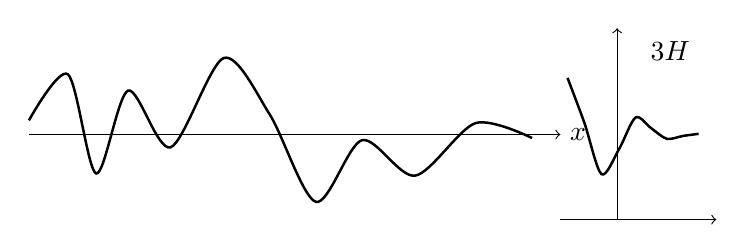
\begin{tikzpicture}[scale=0.9]
\draw[->] (0,0) -- (7.5,0) node[right] {$x$};
\draw[line width=0.9pt] plot[smooth] coordinates {(0.0,0.20) (0.55,0.85) (0.95,-0.55) (1.40,0.62) (2.00,-0.18) (2.75,1.08) (3.40,0.28) (4.05,-0.95) (4.70,-0.08) (5.45,-0.58) (6.30,0.16) (7.10,-0.05)};
\draw[->] (8.3,-1.2) -- (8.3,1.5);
\draw[->] (7.5,-1.2) -- (9.7,-1.2);
\draw[line width=0.9pt] plot[smooth] coordinates {(7.6,0.80) (7.84,0.16) (8.08,-0.56) (8.33,-0.20) (8.56,0.24) (8.78,0.09) (9.00,-0.06) (9.23,-0.02) (9.45,0.01)};
\node at (9.05,1.18) {$3H$};
\end{tikzpicture}
\caption{A cleaned qualitative picture: a field profile built from many frozen wavelengths, together with a damped-oscillation inset.}
\end{figure}

At this point the lecture stresses an important qualitative fact. These are not electromagnetic waves. They are waves of the inflaton field itself. And there is a continuum of wavelengths. In the idealization of an infinite universe, the full field is described not by a discrete sum but by a Fourier integral,
\begin{equation}
\phi(\mathbf{x},t)=\int d^{3}k\, e^{i\mathbf{k}\cdot\mathbf{x}}\phi_k(t),
\end{equation}
up to conventional normalization factors.

Now comes the inflationary production mechanism. If we started with only a fixed set of waves, then eventually they would all be stretched and the field would become smooth. But vacuum fluctuations are always present. New short-wavelength zero-point oscillations continually exist. A short-wavelength mode begins life oscillating rapidly, gets stretched by the expansion, reaches the Hubble scale, freezes, and then another shorter mode takes its place. That one stretches, freezes, and is replaced again. The process repeats continuously.

So the frozen field profile is not arbitrary randomness. It is a superposition of many modes of different wavelengths, shapes, and orientations, each one having gone through the same transition from zero-point oscillation to horizon-sized frozen wave. The lecture does not yet compute a formal power spectrum here. What it gives is the mechanism and the physical scale that controls it.

\section{Falling Off The Cliff: From Frozen Field Noise To Density Perturbations}

We still do not yet have density perturbations. The lecture is explicit on this point: the energy stored directly in the tiny inflaton waves is not enough by itself to explain the observed variations in the energy density. Something else must amplify their effect. That amplification occurs when the inflaton reaches the cliff.

First ignore the noise completely. Then the field has the same value everywhere in space. It slides classically and slowly along the plateau until it reaches the edge. The whole universe then falls off together. The potential energy is converted into particles, heat, and radiation. Inflation ends. The expansion is no longer exponential, and the newly created matter and radiation dilute as the universe continues to expand.

\begin{figure}[htbp]
\centering

\includegraphics[width=0.86\textwidth]{lecture_10_figure_05.png}
\caption{Space-versus-\(\phi\) sketch approaching the inflaton cliff.}
\end{figure}

\begin{figure}[htbp]
\centering
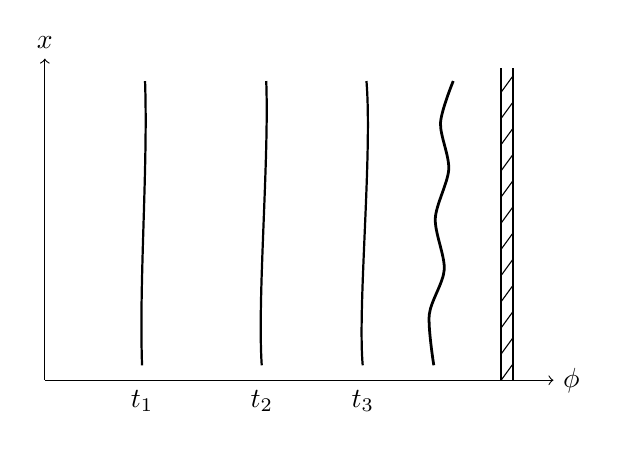
\begin{tikzpicture}[scale=0.95]
\draw[->] (0,0) -- (6.8,0) node[right] {$\phi$};
\draw[->] (0,0) -- (0,4.3) node[above] {$x$};

\draw[line width=0.8pt] (1.30,0.20) .. controls (1.26,1.35) and (1.38,2.85) .. (1.34,4.00);
\draw[line width=0.8pt] (2.90,0.20) .. controls (2.84,1.10) and (3.00,2.95) .. (2.96,4.00);
\draw[line width=0.8pt] (4.25,0.20) .. controls (4.18,0.98) and (4.38,3.02) .. (4.30,4.00);
\draw[line width=1.0pt] plot[smooth] coordinates {(5.20,0.20) (5.14,0.88) (5.34,1.48) (5.22,2.16) (5.40,2.82) (5.29,3.44) (5.46,4.00)};

\draw[line width=1.0pt] (6.10,0.00) -- (6.10,4.18);
\draw[line width=1.0pt] (6.26,0.00) -- (6.26,4.18);
\foreach \y in {0.00,0.35,0.70,1.05,1.40,1.75,2.10,2.45,2.80,3.15,3.50,3.85}{
\draw (6.10,\y) -- (6.26,\y+0.22);
}

\node[below] at (1.30,0) {$t_1$};
\node[below] at (2.90,0) {$t_2$};
\node[below] at (4.25,0) {$t_3$};
\end{tikzpicture}
\caption{A cleaned reconstruction of the lecture's space-versus-\(\phi\) picture. Each nearly vertical profile is the field at a later time, drifting toward the cliff at the right.}
\end{figure}

The blackboard picture is drawn with \(\phi\) on the horizontal axis and space on the vertical axis. At a fixed time, if we ignore fluctuations, the field has the same value everywhere: the profile is a straight vertical line. As time passes, that line drifts toward the cliff.

Now restore the frozen noise. The field is no longer exactly constant across space. It wanders a little. The lecture's image is a line of people walking toward a cliff while trying to keep shoulder to shoulder. A few are a little ahead, a few a little behind. The ones who are ahead go over first.

That timing offset is the real source of the density contrast. A region that goes over first reheats first. Its potential energy is dumped into particles and heat, and then that energy has time to dilute while the universe expands in the post-inflationary era. A nearby region that goes over slightly later reheats later, so when the two are compared, the later region is denser simply because it has had less time to dilute. Thus the tiny field fluctuation is not important because of its own energy; it is important because it shifts the local time at which reheating happens.

This also explains another qualitative statement in the lecture: the slower the roll, the larger the effect. If \(\dot\phi\) is small, then a small spatial variation in \(\phi\) corresponds to a larger time delay before neighboring regions go over the edge. A larger delay means more dilution in the earlier region before the later one reheats. So slower roll produces larger density contrast.

The outcome is a complicated hierarchy of overdense and underdense pockets, nested on many scales. In the lecture this is described as a kind of fractal distribution of energy density. One then writes, in summary,
\begin{equation}
\frac{\delta \rho}{\rho}\sim 10^{-5},
\end{equation}
with the detailed amplitude set by the shape of the potential and the rate of roll.

That is the bridge back to WMAP. The inflaton falls off the cliff at a very early epoch and creates ordinary matter and radiation. The universe then cools for a long time before recombination and transparency. The microwave background is not radiation from time zero; it comes from a shell formed a few hundred thousand years later, after electrons and protons combined into neutral atoms and photons could travel freely. When we look at that shell, we see it passing through a distribution of slightly different densities. Photons from denser regions are redshifted differently from photons from less dense regions, and the temperature map records exactly that structure on the last scattering surface.

Inside that shell, the same density fluctuations continue to evolve. Gravity amplifies them. They become the seeds of galaxy formation and of the large-scale structure seen later in the universe. The lecture also emphasizes that the theory has become highly quantitative: a small set of parameters fits a broad range of angular scales and wave numbers with remarkable precision.

The final caution concerns the largest angular scales. Small-scale anisotropies come in great numbers, so one can do statistics on them. But for the quadrupole and other very low multipoles there is only one sky and therefore only one sample. That is cosmic variance. Large-angle anomalies may be interesting, but the lecture's sober conclusion is that on those scales one must be cautious: with only one universe to observe, there is no way to repeat the experiment.

\section{Summary}

The lecture unfolds in a very deliberate order. First it fixes the hierarchy of scales by distinguishing the universal constants \(c\), \(\hbar\), and \(G\) from the many contingent parameters of low-energy physics, and by building the Planck units from them. Then it states the observational problem: the microwave background is almost isotropic, but its temperature and density fluctuate at the level of \(10^{-5}\), with an approximately scale-invariant pattern.

To explain those fluctuations, the lecture reduces the cosmology to familiar mechanics. The zero-point motion of a harmonic oscillator supplies the primordial quantum noise. The damped harmonic oscillator supplies the vocabulary of underdamped motion, overdamped motion, critical damping, and freezing at nonzero amplitude when the restoring force disappears. The inflaton field in an expanding universe reproduces exactly that system mode by mode:
\begin{equation}
\ddot\phi_k+3H\dot\phi_k+\frac{k^2}{a(t)^2}\phi_k=0.
\end{equation}
As inflation stretches a mode, its restoring force weakens, and it freezes when its physical wavelength reaches the Hubble scale.

That still does not by itself give density perturbations. The final step is the fall off the inflaton cliff. Frozen spatial variations in \(\phi\) make different regions reheat at slightly different times. Earlier regions dilute more, later regions dilute less, and the result is a spatially varying \(\delta\rho/\rho\). Those perturbations later appear on the last scattering surface as the WMAP temperature map and, inside that shell, as the seeds of galaxies and large-scale structure. That is the lecture's central narrative: microscopic quantum fluctuations, stretched by inflation and then amplified by staggered reheating, become the structure of the visible universe.